\documentclass[11pt]{article}
\usepackage[a4paper, portrait, margin=1in]{geometry}
\usepackage{mathtools}
\usepackage{listings}
\usepackage[dvipsnames]{xcolor}
\usepackage{color}
\usepackage{graphicx}
\usepackage[colorlinks=true,urlcolor=blue,linkcolor=gray]{hyperref}


\DeclarePairedDelimiter{\ceil}{\lceil}{\rceil}

\newcommand{\code}[1]{\lstinline[language=Java]{#1}}
\newcommand{\todo}[1]{\fcolorbox{black}{Apricot}{TODO: #1}}
\newcommand{\linkmain}[1]{\href{https://gitlab.inf.ethz.ch/pungast/asl-fall16-project/blob/master/src/main/java/asl/#1.java}{#1}}
\newcommand{\linktest}[1]{\href{https://gitlab.inf.ethz.ch/pungast/asl-fall16-project/blob/master/src/test/java/asl/#1.java}{#1}}

\newcommand{\resultsurl}[1]{\href{https://gitlab.inf.ethz.ch/pungast/asl-fall16-project/blob/master/results/#1}{gitlab.inf.ethz.ch/.../results/#1}}




\begin{document}

\title{Advanced Systems Lab (Fall'16) -- Second
Milestone}

\author{Name: \emph{Taivo Pungas}\\Legi number: \emph{15-928-336}}

\date{
\vspace{4cm}
\textbf{Grading} \\
\begin{tabular}{|c|c|}
\hline  \textbf{Section} & \textbf{Points} \\ 
\hline  1 &  \\ 
\hline  2 &  \\ 
\hline  3 &  \\ 
\hline \hline Total & \\
\hline 
\end{tabular} 
}

\maketitle

\newpage

\section*{Notes on writing the report \small{(remove this page for submission)}}

Before starting to work on this milestone please remember:
\begin{itemize}
\item The prerequisite to a successful completion to this milestone is to have a stable system and also the necessary logging functionalities in place. 
\item Depending on the workload and goal of the experiment, you might need to change the sampling rate from the default level. Make sure to indicate when doing so.
\item The choice of experiment length and repetitions is up to you to decide, please make sure that you do not include warm-up and cool-down phases in the measurements. There are many experiments to run in this milestone, try to make a tradeoff.  
\item We recommend that you have scripts in place to deploy and run experiments.
\item All experiments have to be executed on the Microsoft Azure cloud.
\item When plotting graphs include errors or measures of accuracy whenever possible. 
\item Keep the report compact and concise! The total length should not exceed 20 pages. Log listings are not counted in this length, but all text, figures and tables are. If you have many logs, compress them by experiment and reference the archive instead of the independent files.
\end{itemize}

In this milestone we expect to see the different experiments you ran to exercise the system, and with each experiment we expect a clear description of the system configuration used, the hypothesis on behavior and the explanation of the behavior observed (in terms of the different design decisions taken beforehand) -- \emph{missing either of these for an experiment might make you lose all points for that given experiment!} 

Keep in mind that for a good explanation of the results of an experiment you might have to use one or more methods of data analysis presented in the lecture and in the book. You might have to combine measurements taken in the middleware with the ones at the clients to be able to provide a full picture.

Please feel free to structure the three sections of this report as it makes most sense for your experiments and explanations, but please respect the goal of each section. Also, similarly to the first milestone, include tables and descriptions about your experimental setup before each set of experiments.

\medskip

\pagebreak

% --------------------------------------------------------------------------------
% --------------------------------------------------------------------------------
\section*{Modifications to the middleware}
% --------------------------------------------------------------------------------
% --------------------------------------------------------------------------------
In the last milestone submission, my middleware implemented all functionality as necessary. However, the resource usage was extremely wasteful: each read thread took up nearly 100\% of the resources allocated to them and never went to a sleeping state. This caused more than 10-fold drops in performance when going from $T=1$ to $T=4$ (for $S=5$), and would have made the maximum throughput experiment useless. The changes can be seen on \href{https://gitlab.inf.ethz.ch/pungast/asl-fall16-project/commit/928e9bba132d34ecf9c00936babdd7fa2645e50f}{GitLab}.

To verify that the system is still stable, I re-ran the trace experiment. The throughput and response time are shown in Figures~\ref{fig:trace:throughput} and \ref{fig:trace:responsetime}, and are confirmed to be stable (and throughput is roughly 30\% higher). The Interactive Response Time Law also still holds (to within 0.46\%). For explanations of the figures, see Milestone 1 report.

\begin{figure}[h]
\centering
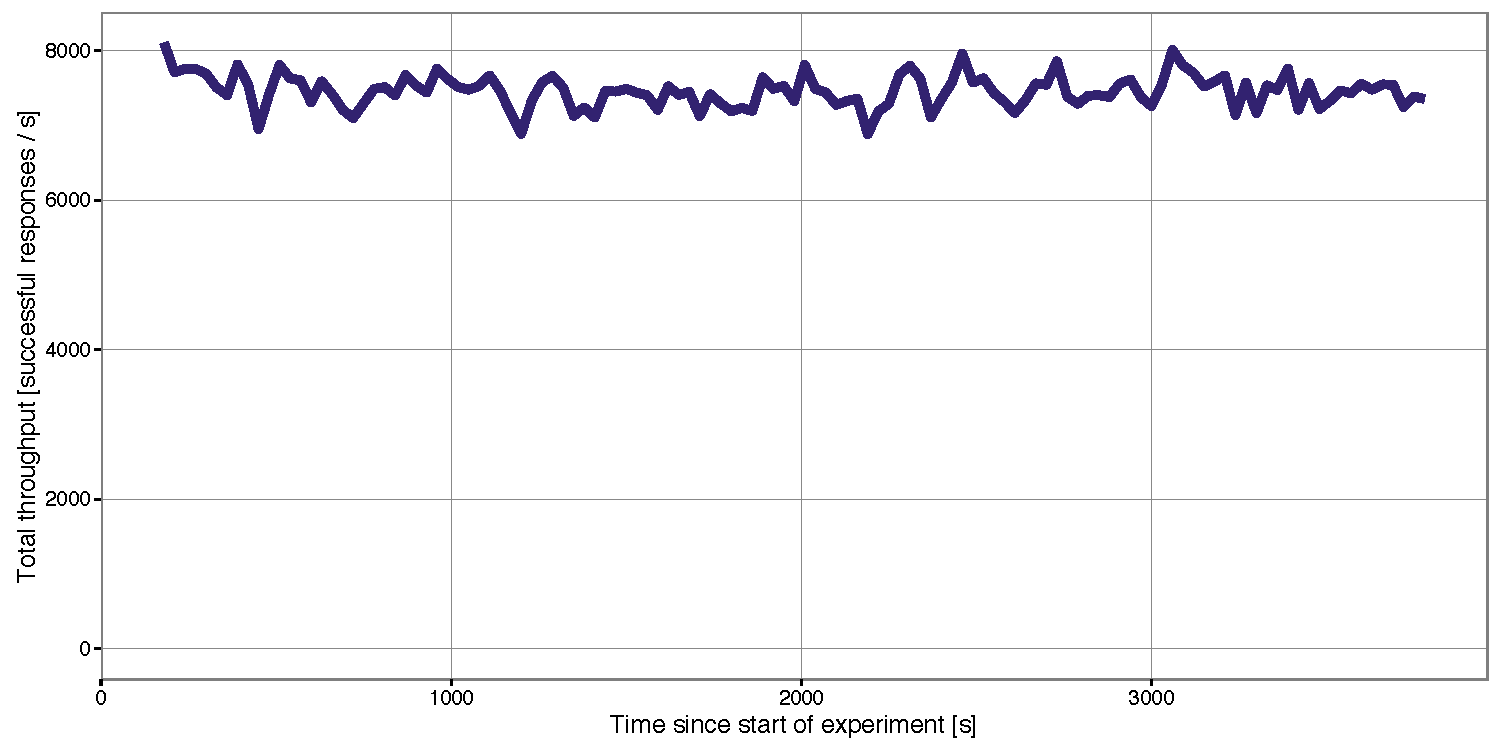
\includegraphics[width=\textwidth]{../results/trace_rep3/graphs/throughput.pdf}
\caption{Throughput trace of the middleware.}
\label{fig:trace:throughput}
\end{figure}

\begin{figure}[h]
\centering
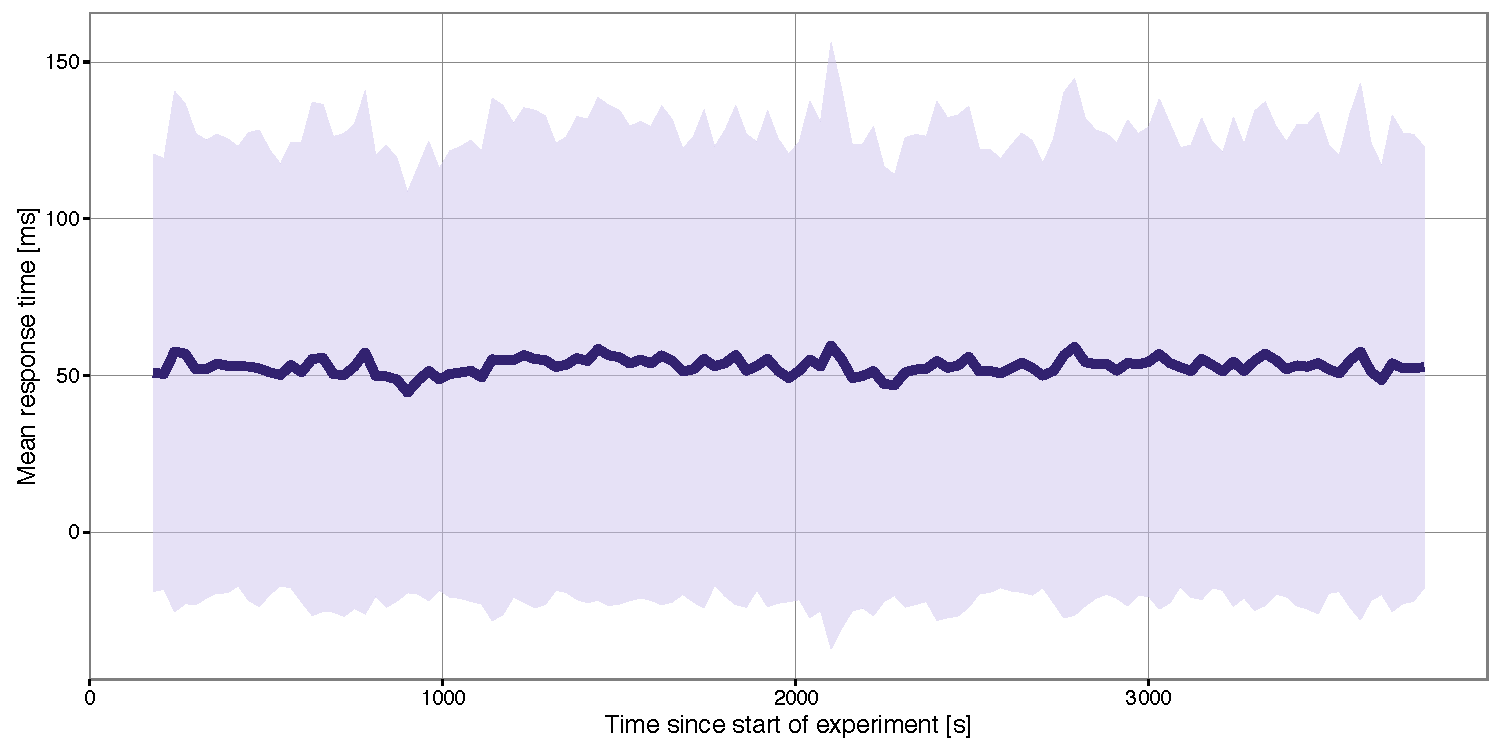
\includegraphics[width=\textwidth]{../results/trace_rep3/graphs/responsetime.pdf}
\caption{Response time trace of the middleware as measured by memaslap.}
\label{fig:trace:responsetime}
\end{figure}


% --------------------------------------------------------------------------------
% --------------------------------------------------------------------------------
\section*{Definitions and setup}
% --------------------------------------------------------------------------------
% --------------------------------------------------------------------------------

In all experiments, the following definitions hold.

\begin{itemize}
\item The \emph{system under test} (SUT) is the middleware together with the connected memcached servers, running on Ubuntu virtual machines in the Azure cloud.
\item \emph{Throughput} is the number of requests the SUT successfully responds to, per unit of time.
\item \emph{Response time} is the time from sending to receiving the request to the SUT including any network latencies, as measured by the client (memaslap).
\end{itemize}

In all experiments, the following holds about the experimental setup:
\begin{itemize}
\item The middleware was run on Basic A4 instances, and both memaslap and memcached were run on Basic A2 instances.
\item The first 2 and last 2 minutes of each experiment were discarded from analyses as warm-up and cool-down time.
\end{itemize}


\clearpage
% --------------------------------------------------------------------------------
% --------------------------------------------------------------------------------
\section{Maximum Throughput}
% --------------------------------------------------------------------------------
% --------------------------------------------------------------------------------

Find the highest throughput of your system for 5 servers with no replication and a read-only workload configuration. What is the minimum number of threads and clients (rounded to multiple of 10) that together achieve this throughput? Explain why the system reaches its maximum throughput at these points and show how the performance changes around these configurations.

Provide a detailed breakdown of the time spent in the middleware for each operation type.

\subsection{Experimental question}

In this section, I will run experiments to find out a) the maximum throughput of the SUT, b) the number of read threads ($T$) in the middleware that achieves this c) the number of virtual clients ($C$) that achieves this.

To this end, I will measure throughput as a function of $T$ and $C$, in 10-second time windows. I will find the maximum sustained throughput of the SUT, i.e. the throughput at which the response time does not increase rapidly with \todo{additional clients}. For each parameter combination, I will run experiments until the 95\% confidence interval (calculated using a two-sided t-test) lies within 5\% of the mean throughput.

\subsection{Hypothesis}

I approximate that the maximum throughput will be 17200 requests per second using 50 read threads in the middleware at a load of 192 to 550 clients.

\paragraph{Number of threads} 
Given that requests spend most of their time ($\sim90\%$ in the trace experiment) waiting in the queue, increasing $T$ will increase throughput. If we reduce the queueing time by a factor of 10, it will no longer be the bottleneck (then waiting for memcached's response -- which takes $\sim9\%$ of response time in the trace experiment -- becomes the bottleneck). Assuming the time spent in the queue scales linearly with the number of read threads, we should increase $T$ 10-fold, i.e. $T=50$ maximises throughput.

\paragraph{Number of clients}
Throughput will be maximised at roughly 110 virtual clients per memcached server, so 550 virtual clients in total. This is based on the fact that in the Milestone 1 baseline experiment, the throughput of a single memcached server without middleware saturated at around 110 virtual clients. It is likely to be an overestimate since the SUT here has an additional part (the middleware) and the baseline experiment did not measure sustained throughput, but 550 clients is a reasonable upper bound. As a lower bound we can use the number of clients in the trace experiment: $3 \cdot 64=192$.

\paragraph{Throughput}
Since in the trace experiment, the throughput was roughly 10300 requests per second, we have a lower bound for the expected throughput. Naively assuming that the throughput of GET requests scales linearly with the number of servers $S$ would yield an expected throughput of $\frac{5}{3} \cdot 10300 = 17200$ requests per second. However, this does not take into account that we will also increase the number of threads (from $T=5$ in the trace experiment). Thus I expect the maximum sustained throughput to be definitely more than 10300 requests per second, and likely to be more than 17200 requests per second.

I predict that the graph of throughput as a function of the number of clients will be similar to Figure~\ref{fig:exp1:hyp:throughput}: rapidly increasing at first, then reaching the knee after which throughput growth is much slower, and then saturating. After saturation, the throughput may fall due to unexpected behaviour in the middleware.

\begin{figure}[h]
\centering
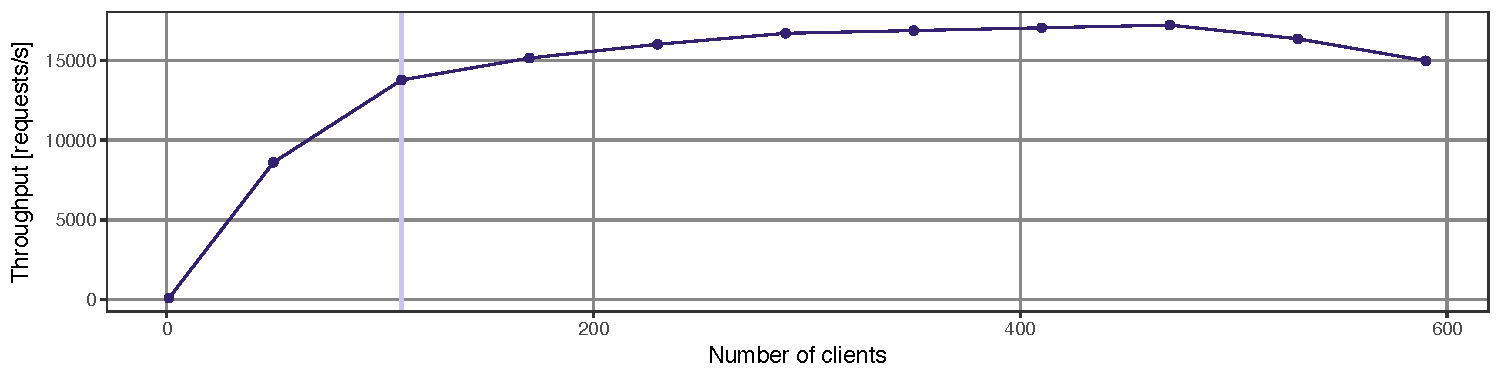
\includegraphics[width=\textwidth]{figures/hypothesis_throughput.pdf}
\caption{Expected graph of throughput as a function of number of clients (for the optimal value of $T$). The vertical line shows the optimal number of clients.}
\label{fig:exp1:hyp:throughput}
\end{figure}

\subsection{Experiments}
\begin{center}
\small{
\smallskip
\begin{tabular}{|c|c|}
\hline Number of servers & 5 \\ 
\hline Number of client machines & $\in \{1, 3\}$ \\ 
\hline Virtual clients & $\in \{1, 36, 72, 144, 216, 288, 360, 432, 504, 576, 648\}$ \\ 
\hline Workload & Key 16B, Value 128B, Writes 0\% \\
\hline Middleware: replication factor & 1 \\ 
\hline Middleware: read threads & $\in\{1, 16, 32, 64\}$ \\ 
\hline Runtime x repetitions & at least 6min x 1; more in some cases \\ 
\hline Log files & \todo{} \\
\hline 
\end{tabular} }
\end{center}

Three client machines were used for all experiments, except for the 1-client experiment, where only one machine was used.

The values of $T$ to test were $T=1$ as the lowest possible value, and then from $T=16$ in multiplicative steps of 2. The reason for the small number of tested values of $T$ is pragmatic: it doesn't require hundreds of experiments and at the same time gives a reasonable approximation of the optimal $T$.

Some parameter combinations did not yield the required confidence interval in the first 6-minute repetition of the experiment. When that was the case, I re-ran the experiment (in some cases for a longer time), thus producing more datapoints and decreasing the confidence interval.

\subsection{Results}
Reporting experiment results.

\begin{figure}[h]
\centering
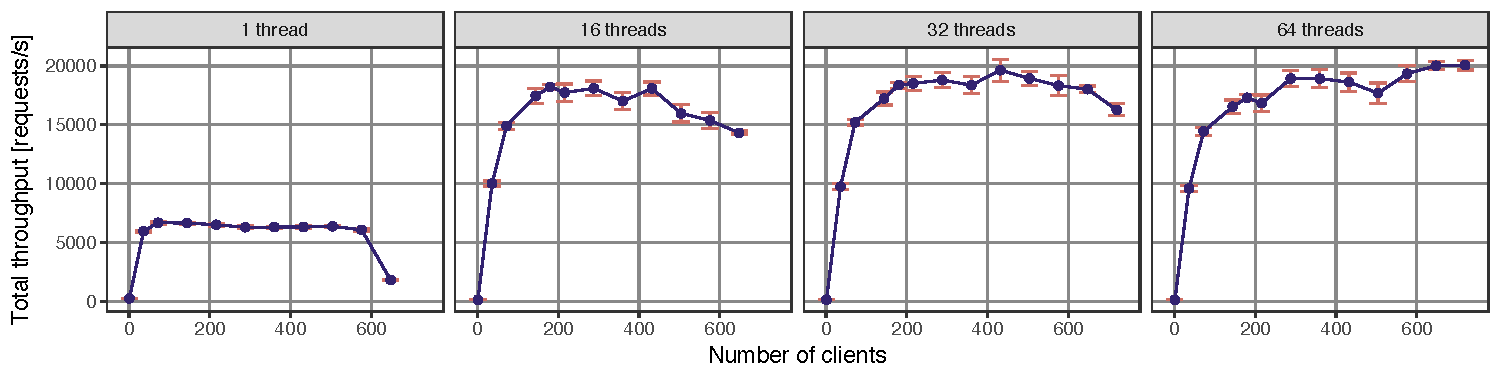
\includegraphics[width=\textwidth]{../results/throughput/graphs/tp_vs_clients.pdf}
\caption{Throughput as a function of $C$ for different values of $T$. Errorbars show the 95\% confidence interval around the mean value which is shown with points connected by lines.}
\label{fig:exp1:res:throughput}
\end{figure}

\begin{figure}[h]
\centering
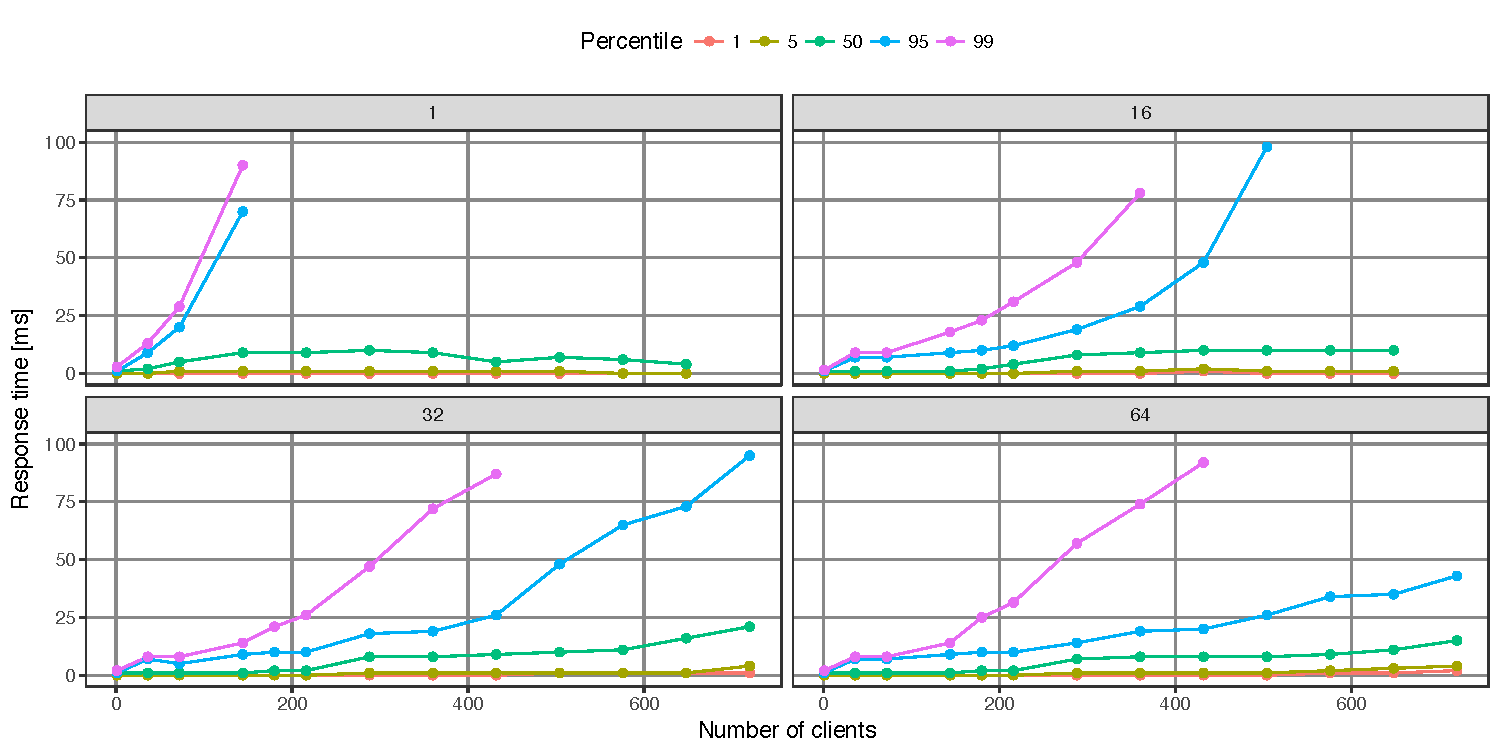
\includegraphics[width=\textwidth]{../results/throughput/graphs/response_time_vs_clients.pdf}
\caption{The 1\%, 5\%, 50\%, 95\% and 99\% percentiles of the response time distribution, as a function of $C$ for different values of $T$. Values above 100ms are not shown.}
\label{fig:exp1:res:responsetime}
\end{figure}

\begin{figure}[h]
\centering
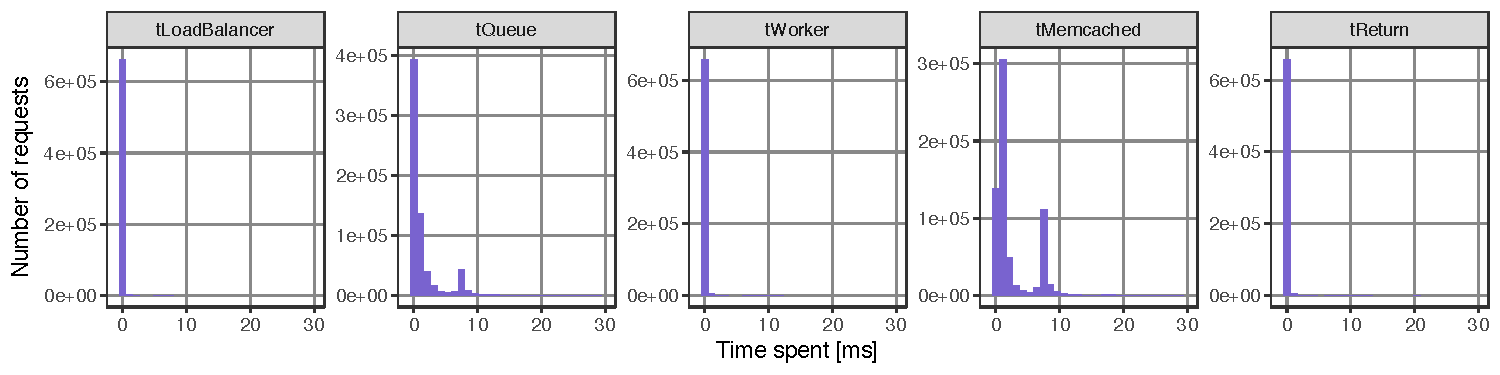
\includegraphics[width=\textwidth]{../results/throughput/graphs/response_time_breakdown.pdf}
\caption{caption \todo{}. Note x axis cut off at 50ms; only GET requests; measured with millisecond accuracy.}
\label{fig:exp1:res:breakdown}
\end{figure}

\begin{tabular}{|c|c|c|r|}
\hline \textbf{Name} & \textbf{Begin timestamp} & \textbf{End timestamp} & \textbf{Mean [ms]} \\
\hline tLoadBalancer & $t_{created}$ & $t_{enqueued}$ & 0.0054 \\
\hline tQueue & $t_{enqueued}$ & $t_{dequeued}$ & 8.49 \\
\hline tWorker & $t_{dequeued}$ & $t_{forwarded}$ & 0.0231 \\
\hline tMemcached & $t_{forwarded}$ & $t_{received}$ & 5.85 \\
\hline tReturn & $t_{received}$ & $t_{returned}$ & 0.0333 \\
\end{tabular}


\todo{Comparison of hypothesis and experiment results.}

Figure \ref{fig:exp1:res:throughput} shows that the highest throughput was achieved using $T=64$ at 720 clients (20100 requests/s), followed by $T=64$ at 648 clients (20000 requests/s) and $T=32$ at 432 clients (19600 requests/s). However, since we are trying to maximise sustained throughput, we also need to look at the response times.

Figure \ref{fig:exp1:res:responsetime} shows the percentiles of the response time distribution for each parameter set. For $(T=64,C=648)$ and $(T=64,C=720)$, both the median response time (green line) and 95\% quantile are significantly higher than for $(T=32, C=432)$. Therefore, we can consider the top two throughputs unsustainable, and declare that the maximal throughput of 19600 requests per second is achieved at 430 clients using 32 threads.




\clearpage
% --------------------------------------------------------------------------------
% --------------------------------------------------------------------------------
\section{Effect of Replication}
% --------------------------------------------------------------------------------
% --------------------------------------------------------------------------------

Explore how the behavior of your system changes for a 5\%-write workload with S=3,5 and 7 server backends and the following three replication factors:
\begin{itemize} 
\item Write to $1$ (no replication) 
\item Write to $\ceil{\frac{S}{2}}$ (half) 
\item Write to all 
\end{itemize}

Answer at least the following questions: Are \texttt{get} and \texttt{set} requests impacted the same way by different setups? If yes/no, why? Which operations become more expensive inside the middleware as the configuration changes? How does the scalability of your system compare to that of an ideal implementation? Provide the graphs and tables necessary to support your claims.


\subsection{Experimental question}

In this section, I will run experiments to find out how the response time of the SUT depends on the number of servers $S$ and replication factor $R$. Additionally, I will investigate whether gets and sets are differently affected by these parameters. Finally, I will find out which operations become more time-consuming as these parameters change.

To this end, I will measure mean response time as a function of $S$ and $R$, and measure how long requests spend in each part of the SUT (based on the timestamps defined in Milestone 1). For each parameter combination, I will run experiments until the 95\% confidence interval (calculated using a two-sided t-test) lies within 10\% of the mean response time.


\subsection{Hypothesis}

\paragraph{Get and set requests}
Get and set requests will not be impacted the same way by different setups.

Get requests will be processed faster as we increase $S$ because the same load will be distributed across more threads. Increasing $R$ will have no effect on get requests because replication is only done for set requests (there may be secondary effects due to e.g. write threads requiring more CPU time, but this should be negligible).

Set requests will be strongly affected by $R$. If $R=1$, set requests will be processed faster for higher $S$ because each request is only written to one server, and for a higher $S$ the same load is distirbuted across more write threads. However, if $R>1$, response time of sets increases due to two factors: a) the request is written serially to $R$ servers, and b) not all $R$ responses are received at the same time. Assuming a) is negligible compared to b), we will observe an increase in the mean response time.

To summarise: for get requests, response time will be independent of $R$ for any fixed $S$. For set requests, response time increases linearly with increasing $R$, and the slope increases with $S$.

\begin{figure}[h]
\centering
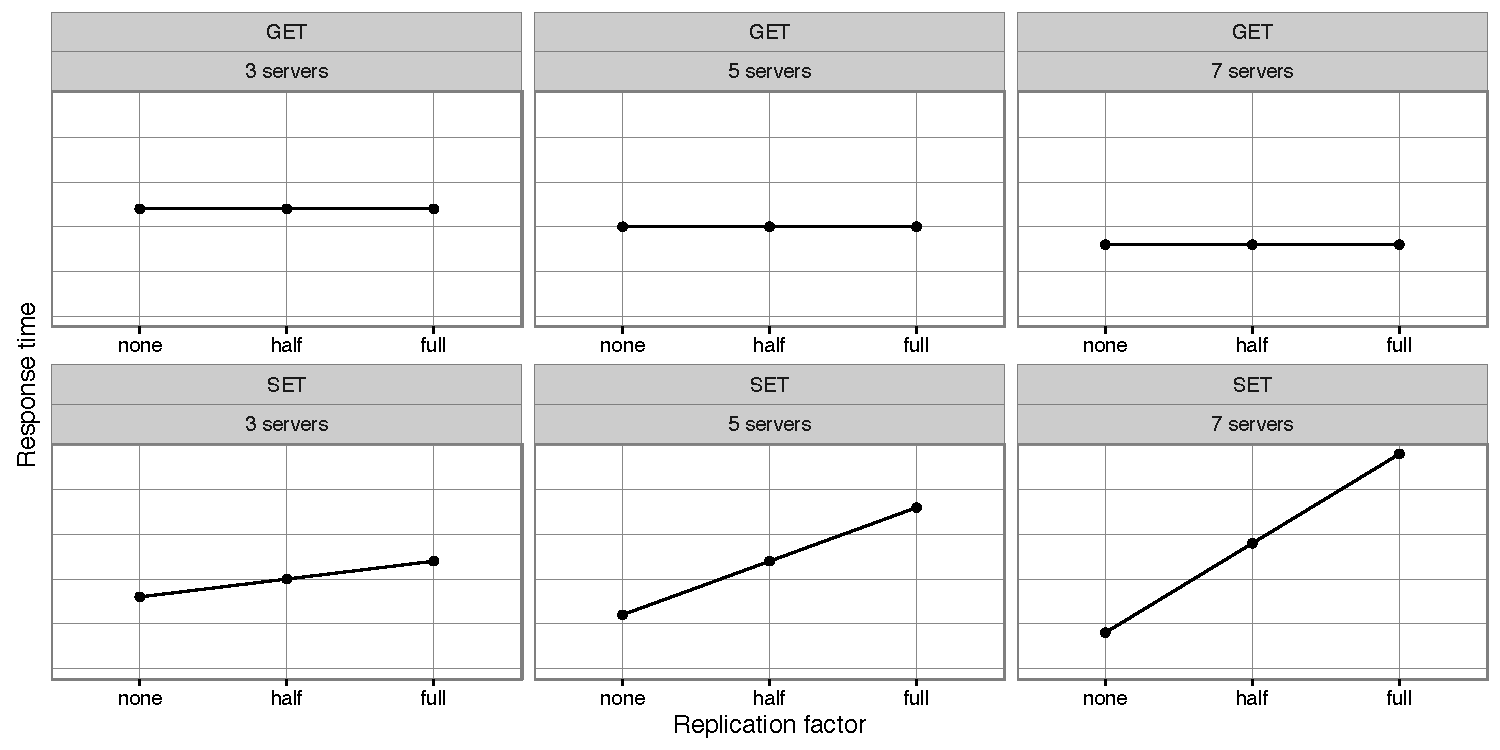
\includegraphics[width=\textwidth]{figures/hypothesis_replication.pdf}
\caption{Expected graph of \todo{}. Mention that y axis is same for all GET subplots and different but constant for all SET subplots.}
\label{fig:exp1:hyp:replication}
\end{figure}


Are get and set requests impacted the same way by different setups? If yes/no, why?

\todo{will be impacted differently}:  gets will improve with increasing S and will be independent of R; sets will get better with increasing S and worse with increasing R

\paragraph{Relative cost of operations}
Which operations become more expensive inside the middleware as the configuration changes?


\paragraph{Scalability}
How does the scalability of your system compare to that of an ideal implementation? 

\todo{Finding how ideal implementation would behave is a good starting point.}

Scale-up? scale out? \todo{check slides}


\begin{itemize}
\item Draw graphs with expected results
\item Even try to predict variance and statistical properties
\item Make bullet points with explanations
\item Use „modeling“ to make hypothesis
\item Formulate a number of questions on what you expect to see, develop a hypothesis around the behavior that is expected, explain the hypothesis, and write it all down
\end{itemize}

\subsection{Experiments}
\begin{center}
\small{
\smallskip
\begin{tabular}{|c|c|}
\hline Number of servers & $\in \{3, 5, 7\}$ \\ 
\hline Number of client machines & 3 \\ 
\hline Virtual clients & \todo{from exp1} \\ 
\hline Workload & Key 16B, Value 128B, Writes 5\% \\
\hline Middleware: replication factor & $\in \{1, ceil(S/2), S\}$ \\ 
\hline Middleware: read threads & \todo{from exp1} \\ 
\hline Runtime x repetitions & 60s x 5 \todo{} \\ 
\hline Log files & \todo{} \\
\hline 
\end{tabular} }
\end{center}

\subsection{Results}
Reporting experiment results. Comparison of hypothesis and experiment results.
How does the scalability of your system compare to that of an ideal implementation?

\todo{table: y axis is S, x axis is R}; in each cell is corresponding response time -- separately for gets and sets?
 

 \clearpage
% --------------------------------------------------------------------------------
% --------------------------------------------------------------------------------
\section{Effect of Writes}
% --------------------------------------------------------------------------------
% --------------------------------------------------------------------------------

In this section, you should study the changes in throughput and response time of your system as the percentage of write operations increases. Use a combination of 3 to 7 servers and vary the number of writes between 1\% and 10\% (e.g. 1\%, 5\% and 10\%). The experiments need to be carried out for the replication factors R=1 and R=all.  

For what number of servers do you see the biggest impact (relative to base case) on performance? Investigate the main reason for the reduced performance and provide a detailed explanation of the behavior of the system. Provide the graphs and tables necessary to support your claims.


\subsection{Experimental question}
\begin{itemize}
\item Define the „system(s) under test“
\item Define what to measure and understand why
\end{itemize}

\subsection{Hypothesis}
\begin{itemize}
\item Draw graphs with expected results
\item Even try to predict variance and statistical properties
\item Make bullet points with explanations
\item Use „modeling“ to make hypothesis
\item Formulate a number of questions on what you expect to see, develop a hypothesis around the behavior that is expected, explain the hypothesis, and write it all down
\end{itemize}

\subsection{Experiments}
\begin{center}
\small{
\smallskip
\begin{tabular}{|c|c|}
\hline Number of servers & $\in \{3, 4, 5, 6, 7\}$ \\ 
\hline Number of client machines & 3 \\ 
\hline Virtual clients / machine & \todo{} \\ 
\hline Workload & Key 16B, Value 128B, Writes $\in \{1\%, 5\%, 10\%\}$ \todo{} \\
\hline Middleware: replication factor & $\in \{1, S\}$ \\ 
\hline Middleware: read threads & \todo{} \\ 
\hline Runtime x repetitions & 60s x 5 \todo{} \\ 
\hline Log files & \todo{} \\
\hline 
\end{tabular} }
\end{center}

\subsection{Results}
Reporting experiment results. Comparison of hypothesis and experiment results.


\pagebreak

\section*{Logfile listing}

\begin{tabular}{|c|l|}
\hline \textbf{Short name }& \textbf{Location} \\ 
\hline baseline-m*-c*-r* & \href{https://gitlab.inf.ethz.ch/pungast/asl-fall16-project/blob/master/results/baseline}{gitlab.inf.ethz.ch/.../results/baseline/baseline\_memaslap*\_conc*\_rep*.out} \\ 
\hline trace-ms4 & \resultsurl{trace\_rep3/memaslap4.out} \\ 
\hline 
\end{tabular} 
 
\end{document}